\documentclass[11pt,a4paper]{article}

% ---- packages ----
\usepackage[margin=1in]{geometry}
\usepackage{times}
\usepackage{setspace}
\usepackage{graphicx}
\usepackage{booktabs}
\usepackage{tabularx}
\usepackage{array}
\usepackage{amsmath}
\usepackage{amssymb}
\usepackage{hyperref}
\usepackage{xcolor}
\usepackage{caption}
\usepackage{subcaption}
\usepackage{float}
\usepackage{enumitem}
\usepackage[numbers,sort&compress]{natbib}
\usepackage{doi}

\hypersetup{
  colorlinks=true,
  linkcolor=black,
  citecolor=blue!50!black,
  urlcolor=blue!50!black
}

\onehalfspacing
\setlength{\parskip}{0.35em}

\title{\textbf{Dual Seeding under a Geographic Paradox:\\
Hospital-Associated SARS-CoV-2 in Hong Kong after Visit-Schedule Relaxation}}
\author{
Shen Ruililin\\[0.35em]
\small Laidlaw Scholars Programme, The University of Hong Kong\\[0.6em]
\small Companion research note to Shen et al.\ (2026)\\
\small\textit{Exploratory genomic-epidemiologic reanalysis --- first draft}
}
\date{11 July 2026}

\begin{document}
\maketitle

\begin{abstract}
\noindent
\textbf{Background.}
After Hong Kong relaxed hospital visitation in May 2022, nosocomial SARS-CoV-2 clusters re-emerged amid Phase-2 community transmission.
A recent multihospital genomic study characterised ward-level transmission and found no independent association between community mobility and community-to-hospital viral introductions.
Here we ask two further questions that study left open: (i)~whether ward outbreaks are initiated by a single dominant route or by \emph{dual seeding}, and (ii)~why sequenced hospital-associated infections concentrate in New Territories (NT) clusters despite lower population and hospital geographic density.

\textbf{Methods.}
We reanalysed the published hospital-associated sequence plot table ($n=162$ cases; 17 anonymised hospitals; 28~May--18~Aug~2022), linked cases to Hospital Authority (HA) clusters, classified ward-level initiation pathways from first detection dates, and standardised burden by HA beds, inpatient discharges, and patient-days (FY2021--22).
District census data quantified catchment density.
Official HA nosocomial press bulletins were mined for an ascertainment footprint (presence of clusters by hospital/cluster).

\textbf{Results.}
Staff/outpatient-first and inpatient-first pathways both contributed substantial burden (48 vs 54 cases among ordered dual-type wards); pathway mix did not differ detectably between NT and urban clusters.
NTWC+NTEC comprised 82.7\% of sequenced hospital-associated cases despite $\sim$0.27$\times$ mean population density and $\sim$0.20$\times$ hospital geographic density relative to urban clusters in the sample.
The NT excess survived standardisation by beds ($\sim$5.7$\times$), discharges ($\sim$6.9$\times$), and patient-days ($\sim$5.7$\times$).
Kowloon East provided a negative control (low hospital density, low sequenced burden).
Official bulletins mentioned Kowloon Central Cluster hospitals that are absent from the sequenced table, indicating uneven genomic coverage; NT/psychiatric hospitals (notably Castle Peak) were also prominent in public reporting.

\textbf{Conclusions.}
Hospital-associated SARS-CoV-2 in this window was dually seeded and geographically structured, not a simple function of urban density or citywide mobility.
Throughput denominators do not erase the NT excess; ascertainment is uneven and must temper causal language.
The findings support ward- and case-mix-targeted infection prevention---including long-stay/psychiatric settings---alongside visitor screening.
\end{abstract}

\noindent\textbf{Keywords:}
SARS-CoV-2; nosocomial transmission; dual seeding; geographic concentration; New Territories; genomic epidemiology; Hong Kong

\section{Introduction}

Hong Kong's fifth COVID-19 wave forced a transition from near-elimination to managed endemicity.
In May 2022, authorities phased in relaxed hospital visitation while community incidence rebuilt into Phase~2 of the fifth wave~\cite{shen2026hai}.
Understanding how SARS-CoV-2 entered and spread within hospitals during that transition matters for future respiratory-pathogen preparedness: visitation has clear benefits for patients~\cite{shen2026hai}, yet wards remain vulnerable when community prevalence is high.
Hong Kong hospitals faced intense Omicron pressure even with high healthcare-worker vaccination coverage~\cite{wong2022hcw}, and multi-bedded cubicle design facilitated onward spread despite enhanced infection-prevention measures~\cite{wee2022cubicles}.

International genomic epidemiology has repeatedly shown that hospital SARS-CoV-2 dynamics are multi-route rather than single-pathway.
Combined epidemiological--genomic reconstructions across two UK pandemic waves found shifting contributions of staff--patient transmission and strong location hotspots~\cite{lindsey2022natcomms}.
Contact-aware analyses demonstrate that healthcare-worker (HCW) location data reveal cryptic links missed by patient-only tracing~\cite{ellingford2021elife}, while on-demand hospital genomics documents multiple coexisting transmission modes and can refute epidemiologically suspected nosocomial links~\cite{benoit2023ash}.
At the same time, many epidemiologically labelled ``outbreaks'' comprise multiple genomic introductions rather than a single chain~\cite{haanappel2023aric}.
These findings motivate an explicit dual-seeding taxonomy---staff/outpatient bridges versus inpatient introductions---rather than assuming a single dominant entry route.

Case-mix further structures risk.
Closed psychiatric and long-term mental-health settings have recorded extreme attack rates and IPC challenges poorly served by acute-ward protocols~\cite{chun2020frontiers,rovers2020aric,kim2023medicina}.
Geographic patterning of facility outbreaks is real but not reducible to urban density alone: some analyses find higher outbreak odds outside the densest metropolitan cores after adjustment~\cite{doggui2025scirep}, whereas other systems show capital-region concentration~\cite{espenhain2023eurgeriatr}.
Against that backdrop, a New Territories excess of sequenced hospital-associated infections in Hong Kong is scientifically interesting precisely because NT catchments are \emph{less} dense.

Shen et al.\ sequenced 162 genomes linked to 29 suspected ward clusters across 17 public hospitals (28~May--18~August~2022), confirmed 18 nosocomial clusters (126 genomes), showed predominantly intraward transmission without resolved interward spread, and inferred more community$\to$hospital than hospital$\to$community Markov jumps~\cite{shen2026hai}.
After adjusting for time trends, generalised additive models found no significant association between introduction rates and standard mobility indices~\cite{shen2026hai}.

Two gaps remain.
First, \emph{how} wards are seeded: the parent analysis noted phylogenetic staff-before-inpatient order in only 2/18 confirmed clusters~\cite{shen2026hai}, but a broader temporal taxonomy of staff/outpatient versus inpatient first detections has not been quantified across all investigated wards.
Second, \emph{where} burden concentrates: sequenced hospital-associated infections are heavily skewed toward New Territories West and East clusters (NTWC, NTEC), yet New Territories districts are less densely populated and have fewer hospitals per land area than urban catchments---a pattern that challenges naive ``dense city, more hospital outbreaks'' intuition.

\paragraph{Research questions.}
\begin{enumerate}[leftmargin=1.4em,itemsep=0.2em]
  \item Are hospital-associated clusters in this window consistent with a single dominant initiation route, or with \textbf{dual seeding} (staff/outpatient bridges and inpatient introductions)?
  \item Does the New Territories concentration of sequenced hospital-associated infections persist after standardisation by hospital throughput, and can density or ascertainment explain it?
\end{enumerate}

\paragraph{Contribution.}
This companion note does not re-estimate phylogenies.
It delivers a manuscript-ready descriptive and standardised reanalysis: a dual-seeding taxonomy; a quantified density paradox with negative controls; admissions/patient-day denominators; and an honest ascertainment audit against public HA bulletins.

\section{Methods}

\subsection{Data sources}
\begin{itemize}[leftmargin=1.4em,itemsep=0.15em]
  \item \textbf{Hospital-associated cases.} Anonymised plot table from the parent study ($n=162$ sequenced cases; hospitals A--Q; HA cluster labels; ward; case type; lineage; date)~\cite{shen2026hai}.
  \item \textbf{HA capacity and throughput.} Beds (31~Mar~2022) and FY2021--22 inpatient discharges and patient-days from HA Statistical Report cluster extracts~\cite{ha2022stat}.
  \item \textbf{Catchment demography.} 2021 Population Census district populations and land areas, mapped to conventional HA cluster catchments~\cite{census2021,legco2017}.
  \item \textbf{Official reporting footprint.} HA press releases on info.gov.hk announcing nosocomial COVID-19 clusters during the study window (presence of hospitals in nosocomial tables/narratives).
  \item \textbf{Parent coverage anchor.} Confirmed genomic clusters represented 51.9\% of officially reported nosocomial cases in the window~\cite{shen2026hai}.
\end{itemize}

\subsection{Dual-seeding classification}
For each hospital--ward combination, we recorded the earliest detection date by case type.
Pathways were labelled:
\textit{staff\_first}, \textit{inpatient\_first}, \textit{same\_day}, \textit{staff\_only}, or \textit{inpatient\_only}.
``Staff'' here aggregates Outpatient/Staff in the plot table.
This is a \emph{temporal first-detection} definition, complementary to---not identical with---the parent paper's phylogenetic staff-index criterion~\cite{shen2026hai}.
Among wards with both staff and inpatient detections and a clear order, we tested NT versus urban pathway mix with Fisher's exact test.

\subsection{Geographic and density metrics}
HA clusters were grouped as New Territories (NTWC, NTEC) versus urban clusters present in the sequenced table (KWC, KEC, HKEC).
Population density used catchment population (2017 planning projection) divided by core district land area.
Hospital and bed geographic density used HA facility counts and beds per 100~km$^2$ of core land area.
Islands/Lantau splits for HKEC/KWC were excluded from core land area (conservative for urban density).

\subsection{Denominator standardisation}
Sequenced hospital-associated case counts were standardised as:
cases per 1{,}000 beds; per 100{,}000 annual inpatient discharges; and per 100{,}000 annual inpatient patient-days.
Annual FY2021--22 throughput is an imperfect proxy for an 83-day window; we therefore emphasise relative NT/urban ratios rather than absolute window incidence.
Mentally-ill patient-day share was computed as a case-mix marker.

\subsection{Ascertainment audit}
Because the parent supplement Table~S3 (official case totals by hospital) was not recoverable in this environment (curated Excel gitignored; publisher supplement inaccessible), we did \emph{not} invent cluster-level coverage fractions from daily press tables (which are incremental and reconstruct only a small fraction of the implied $\sim$243 official cases).
Instead we contrast \textbf{presence}: HA clusters appearing in official nosocomial bulletins versus those appearing in the sequenced plot table, anchored by the published 51.9\% overall coverage statistic~\cite{shen2026hai}.

\subsection{Ethics and anonymisation}
Analyses use aggregated, anonymised hospital codes as in the parent study.
HA cluster labels provide geographic context already used publicly~\cite{shen2026hai}.

\section{Results}

\subsection{Dual seeding is a shared mechanism}
Across 29 wards, ordered dual-type pathways contributed 48 staff/outpatient-first and 54 inpatient-first cases; same-day detections added 24 (Table~\ref{tab:pathways}).
Staff-only and inpatient-only wards contributed smaller burdens.
Fisher's exact test comparing NT versus urban wards for staff-first versus inpatient-first yielded OR~$=0.33$, $p=0.56$ ($n=13$ wards): no evidence of different dominant routes by region.
Among inpatients with known admission-to-positive interval (API), 74/90 (82\%) had API~$\ge 3$~days, consistent with substantial in-hospital acquisition once infection is inside the ward~\cite{shen2026hai}.

\begin{table}[H]
\centering
\caption{Ward-level temporal initiation pathways (sequenced hospital-associated cases).}
\label{tab:pathways}
\begin{tabular}{lrr}
\toprule
Pathway & Wards & Cases \\
\midrule
Staff/outpatient first & 6 & 48 \\
Inpatient first & 7 & 54 \\
Same day & 3 & 24 \\
Staff/outpatient only & 5 & 15 \\
Inpatient only & 8 & 21 \\
\bottomrule
\end{tabular}
\end{table}

\begin{figure}[H]
\centering
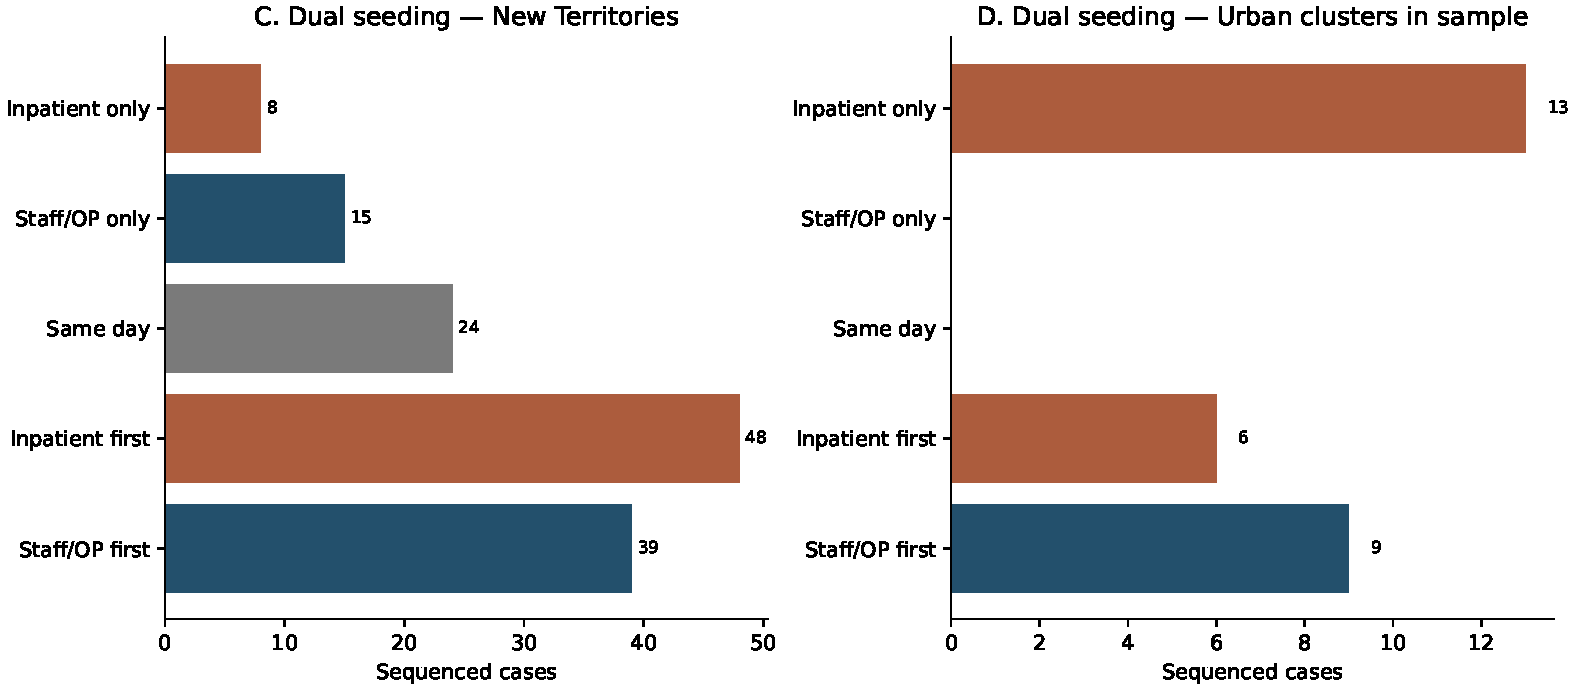
\includegraphics[width=0.98\textwidth]{figures/fig_dual_seeding_by_region.pdf}
\caption{Dual-seeding composition by region (case counts). Staff/outpatient-linked and inpatient-linked routes both matter in New Territories and urban clusters in the sample.}
\label{fig:dual}
\end{figure}

\subsection{Geographic concentration despite lower density}
NTWC+NTEC accounted for 134/162 (82.7\%) sequenced hospital-associated cases.
Mean catchment population density for NT clusters was $\sim$0.27$\times$ that of urban in-sample clusters; hospitals per 100~km$^2$ $\sim$0.20$\times$; beds per 100~km$^2$ $\sim$0.29$\times$ (Figure~\ref{fig:density}).
Kowloon East Cluster (KEC) had similarly low hospital geographic density ($\sim$2 per 100~km$^2$) but low sequenced burden---a negative control showing that low density is not sufficient for high observed hospital-associated infection.

\begin{figure}[H]
\centering
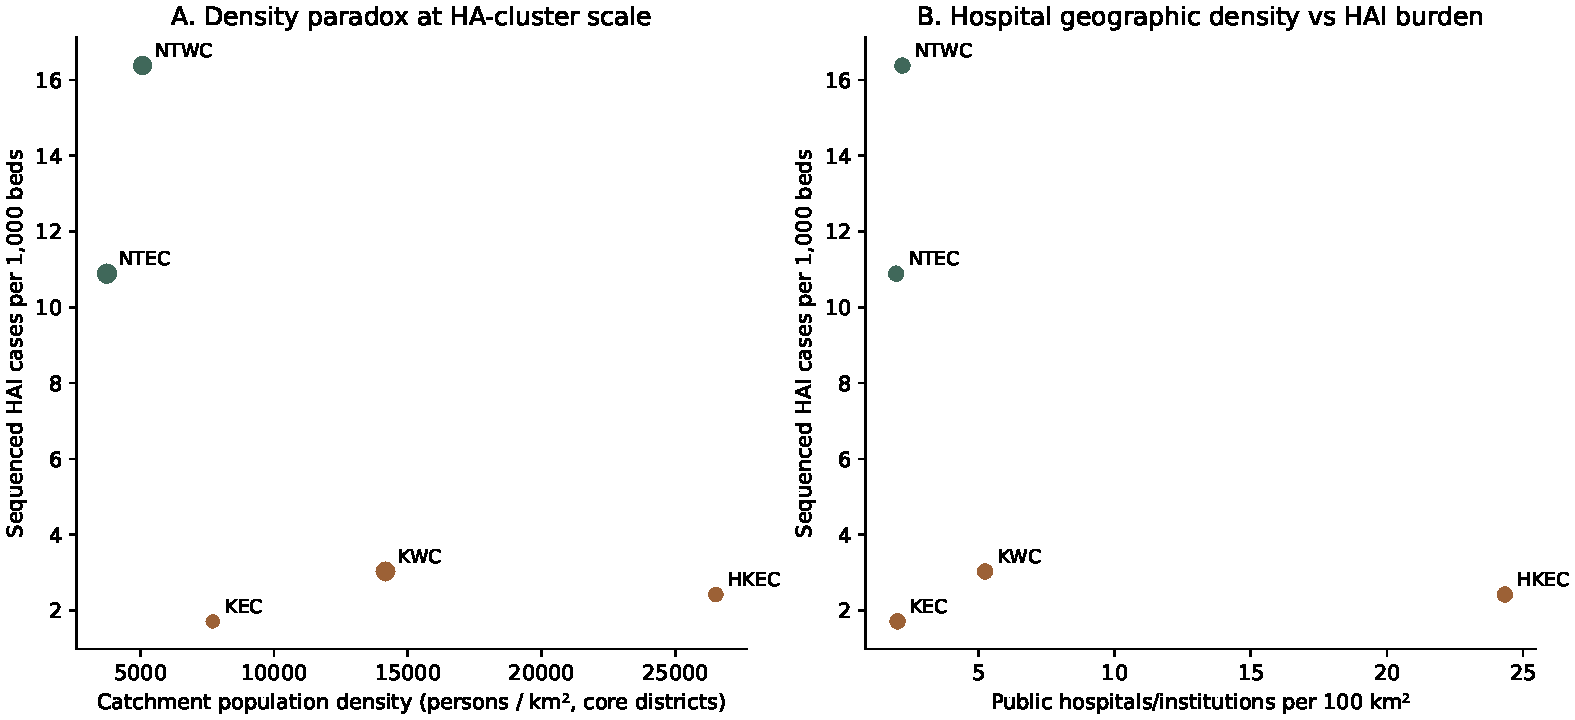
\includegraphics[width=0.98\textwidth]{figures/fig_density_paradox.pdf}
\caption{Density paradox at HA-cluster scale. New Territories clusters (green) combine lower population and hospital geographic density with higher sequenced hospital-associated infection rates per 1{,}000 beds.}
\label{fig:density}
\end{figure}

\subsection{The NT excess survives throughput denominators}
Standardising by beds, discharges, and patient-days left a several-fold NT excess relative to urban in-sample clusters (Table~\ref{tab:denom}; Figure~\ref{fig:denom}):
approximately 5.7$\times$ per 1{,}000 beds, 6.9$\times$ per 100{,}000 discharges, and 5.7$\times$ per 100{,}000 patient-days (means of cluster-level rates).
NTWC showed the highest mentally-ill patient-day share (19.2\% of cluster patient-days), linking geography to long-stay case-mix (Figure~\ref{fig:psych}).
All 22 BA.5.6 sequences in the plot table arose from a single hospital ward with almost exclusively API~$\ge 3$ inpatients---a deep nosocomial signature inside NTWC~\cite{shen2026hai}.

\begin{table}[H]
\centering
\caption{Sequenced hospital-associated infections standardised by HA throughput (FY2021--22).}
\label{tab:denom}
\resizebox{\textwidth}{!}{%
\begin{tabular}{lrrrrrr}
\toprule
Cluster & Cases & Beds & Discharges & Patient-days & /1k beds & /100k discharges \\
\midrule
NTWC & 78 & 4{,}762 & 140{,}388 & 1{,}331{,}433 & 16.38 & 55.56 \\
NTEC & 56 & 5{,}144 & 163{,}397 & 1{,}311{,}078 & 10.89 & 34.27 \\
KWC  & 15 & 4{,}953 & 201{,}096 & 1{,}416{,}390 & 3.03 & 7.46 \\
HKEC & 8 & 3{,}307 & 102{,}190 & 822{,}971 & 2.42 & 7.83 \\
KEC  & 5 & 2{,}922 & 114{,}909 & 809{,}758 & 1.71 & 4.35 \\
KCC  & 0 & 6{,}005 & 199{,}221 & 1{,}599{,}173 & 0 & 0 \\
HKWC & 0 & 3{,}076 & 103{,}370 & 635{,}637 & 0 & 0 \\
\bottomrule
\end{tabular}}
\end{table}

\begin{figure}[H]
\centering
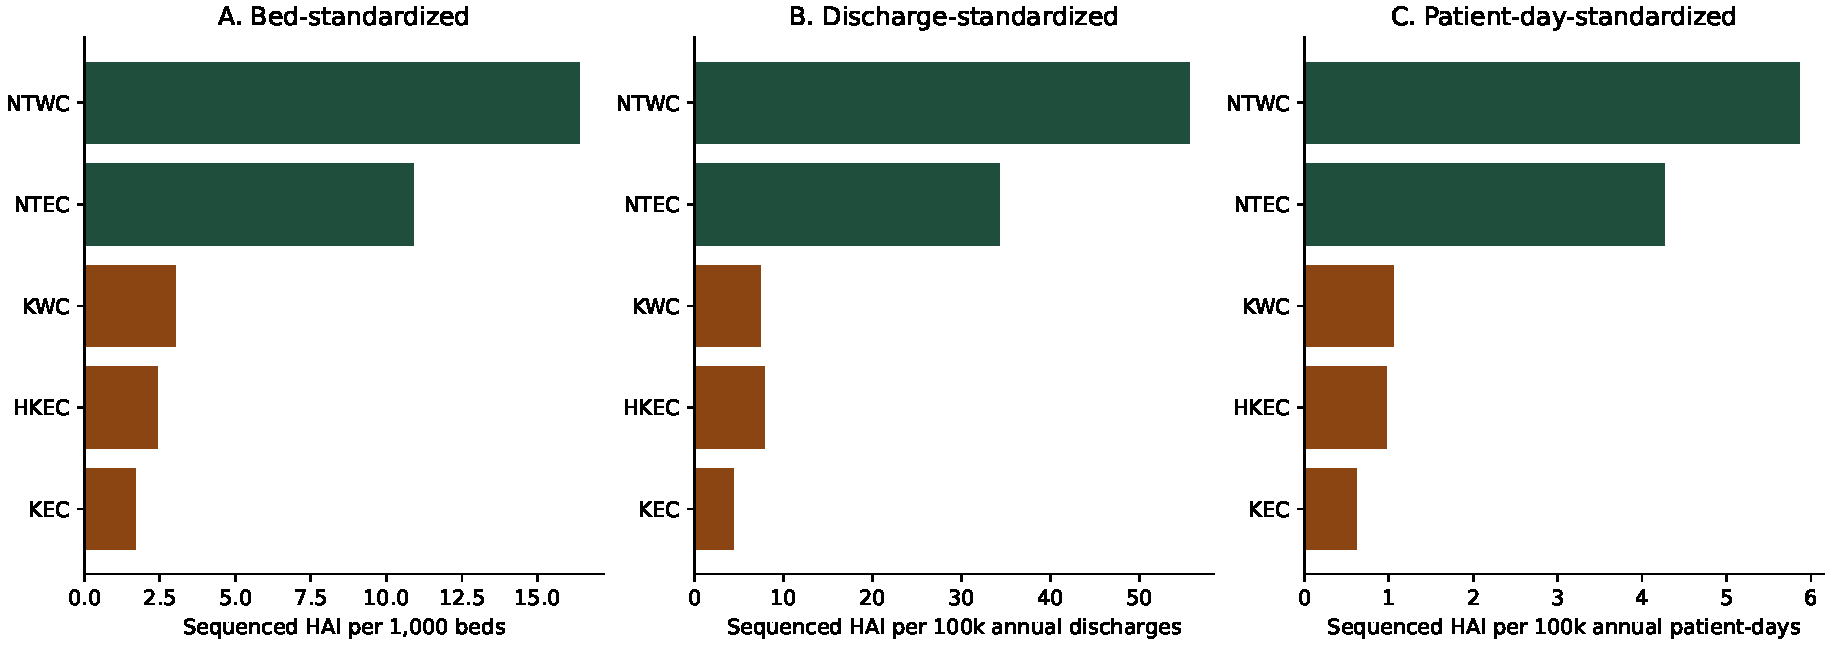
\includegraphics[width=0.98\textwidth]{figures/fig_denominator_standardization.pdf}
\caption{Sequenced hospital-associated infection rates under three denominators. New Territories clusters remain elevated after bed, discharge, and patient-day standardisation.}
\label{fig:denom}
\end{figure}

\begin{figure}[H]
\centering
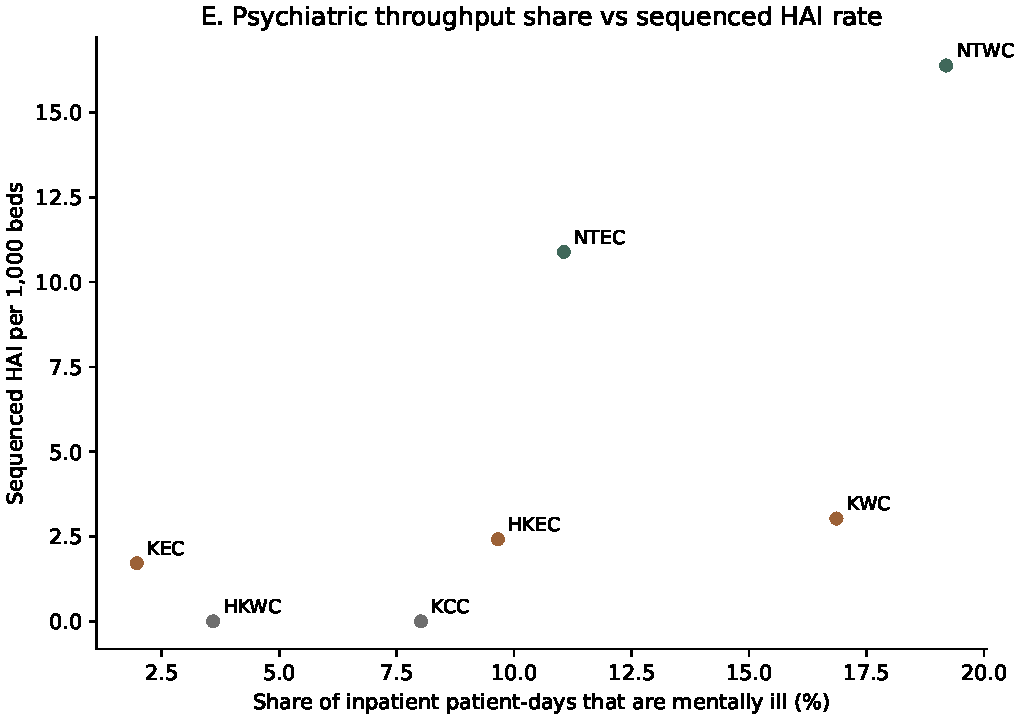
\includegraphics[width=0.72\textwidth]{figures/fig_psych_share_vs_hai.pdf}
\caption{Mentally-ill patient-day share versus sequenced hospital-associated infection rate. NTWC combines high psychiatric throughput share with the highest bed-standardised rate.}
\label{fig:psych}
\end{figure}

\subsection{Ascertainment is uneven---and must be stated plainly}
Parent-study confirmed clusters covered 51.9\% of official nosocomial cases overall~\cite{shen2026hai}.
Public HA bulletins during the window mentioned hospitals in \emph{all seven} HA clusters, including Kowloon Central and Hong Kong West---yet those two clusters contribute zero cases to the sequenced plot table (Figure~\ref{fig:asc}).
Conversely, NTWC (especially Castle Peak Hospital) and NTEC appear in both official bulletins and the sequenced table.
Daily bulletin tables are incremental and cannot replace Table~S3 cumulative counts; we therefore claim a \textbf{presence contrast}, not cluster-specific coverage percentages.

\begin{figure}[H]
\centering
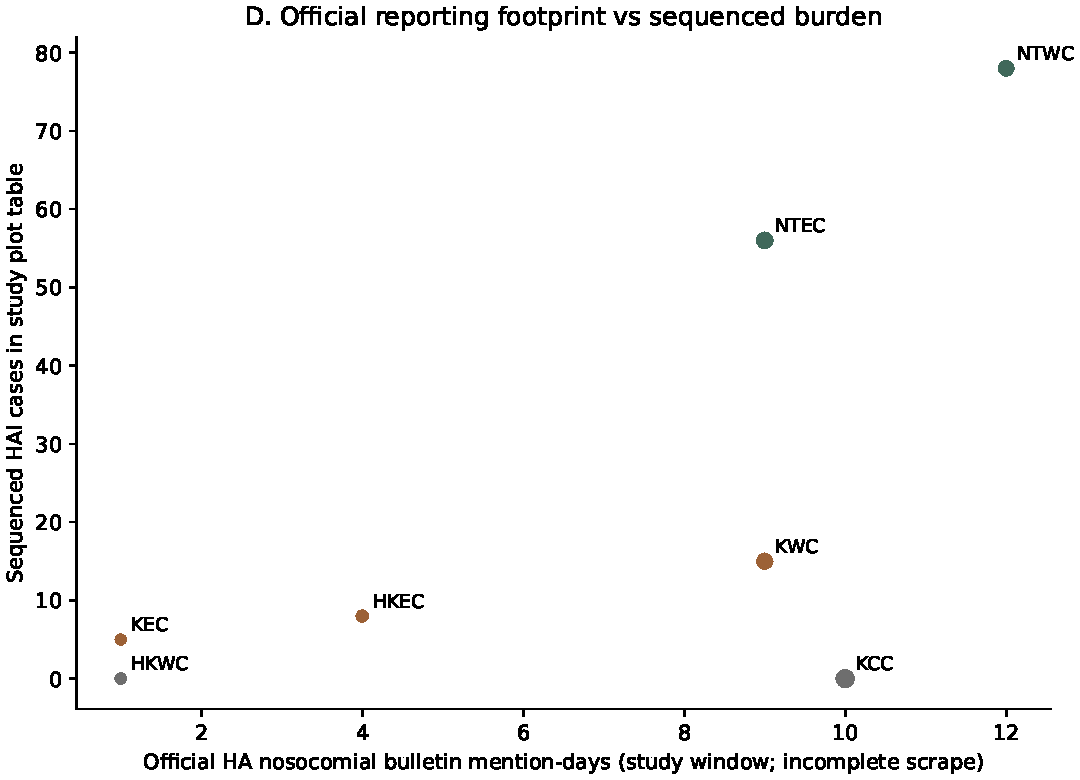
\includegraphics[width=0.75\textwidth]{figures/fig_ascertainment_mentions_vs_sequences.pdf}
\caption{Official nosocomial bulletin mention-days versus sequenced hospital-associated cases. KCC lies on the $x$-axis (mentioned, not sequenced in the plot table), illustrating uneven genomic coverage.}
\label{fig:asc}
\end{figure}

\section{Discussion}

\subsection{What the dual-seeding result changes}
If wards were seeded almost only by visitors, policy could focus narrowly on visitation rules.
Our temporal taxonomy shows staff/outpatient-first and inpatient-first routes both carry large case burdens, and the mix is shared across NT and urban clusters.
That result sits comfortably with international evidence that HCW--patient networks and multi-route transmission are the rule rather than the exception~\cite{lindsey2022natcomms,ellingford2021elife,benoit2023ash}, and with the parent paper's caution that healthcare workers with routine community exposure are plausible bridges~\cite{shen2026hai}.
It also preserves a role for incubating admissions despite mandatory admission screening.
Phylogenetic staff-index events were rarer (2/18 confirmed clusters)~\cite{shen2026hai}; temporal first detection is more sensitive and should be reported as a complementary definition---especially because genomic studies often show that single epidemiological ``outbreaks'' hide multiple introductions~\cite{haanappel2023aric,benoit2023ash}.

\subsection{Why the density paradox matters}
The NT excess is the opposite of a density-driven urban story.
Lower population and hospital geographic density, yet higher standardised sequenced burden, redirects attention to hospital case-mix (long-stay and psychiatric capacity), IPC implementation, and sampling---not skyline density.
Literature on facility outbreaks already warns that geography matters in inconsistent directions: capital-region concentration in some systems~\cite{espenhain2023eurgeriatr}, elevated odds outside the densest core in others~\cite{doggui2025scirep}.
KEC's low density with low burden prevents the lazy inference that ``sparse geography causes outbreaks.''
Instead, NTWC's high mentally-ill patient-day share and the BA.5.6 single-ward deep outbreak echo the well-documented vulnerability of psychiatric and long-stay settings~\cite{chun2020frontiers,rovers2020aric,kim2023medicina}.

\subsection{Denominators versus ascertainment}
Admissions and patient-day standardisation were the cleanest quantitative tests available without hospital-level window admissions.
They fail to wash out NT concentration.
Sequencing-effort tip counts from the study trees are largely circular with the sample itself and were not used as independent proof.
The bulletin presence contrast shows under-representation of some urban clusters (notably KCC) in the sequenced table: NT excess is unlikely to be \emph{only} artefact, but it is also not fully separable from ascertainment without Table~S3 hospital totals.
This limitation is itself a finding about surveillance design: genomic programmes that follow the loudest clusters can reify geographic narratives unless coverage is audited against independent official registries~\cite{shen2026hai,benoit2023ash}.

\subsection{Limitations}
\begin{enumerate}[leftmargin=1.4em,itemsep=0.15em]
  \item Sequenced hospital-associated cases $\neq$ complete nosocomial incidence.
  \item Annual throughput approximates an 83-day window.
  \item Temporal dual-seeding $\neq$ phylogenetic index.
  \item Official bulletin mining is incomplete relative to curated Table~S3.
  \item Catchment populations are planning estimates, not closed cohorts.
\end{enumerate}

\subsection{Implications}
During high community prevalence, protecting hospitals requires more than citywide mobility management (already null in the parent GAM)~\cite{shen2026hai}.
Practical levers include: (i)~dual attention to staff/community bridges \emph{and} admission pathways~\cite{lindsey2022natcomms,ellingford2021elife}; (ii)~heightened, psychiatry-adapted IPC in long-stay settings~\cite{rovers2020aric,kim2023medicina}; (iii)~genomic surveillance designed for even cluster coverage, not only the loudest outbreaks.

\section{Conclusion}
Hospital-associated SARS-CoV-2 in Hong Kong's post-relaxation window was \textbf{dually seeded} and \textbf{geographically structured}.
New Territories concentration persists after throughput standardisation and sits inside a density paradox that urban intuition does not explain.
Ascertainment is uneven; recovering hospital-level official totals remains the highest-value upgrade.
Until then, the evidence supports ward- and case-mix-targeted prevention over density- or mobility-centric narratives alone.

\section*{Data and code}
Analysis scripts and tabulated outputs are in the project repository
(\texttt{scripts/4.dual\_seeding\_geography.py},
\texttt{scripts/5.denominators\_ascertainment.py}, and \texttt{analysis/}).
Parent genomic methods and primary figures are described in Shen et al.~\cite{shen2026hai}.

\section*{Competing interests}
None declared for this companion reanalysis draft.

\section*{Acknowledgements}
Prepared under the Laidlaw Scholars Programme, The University of Hong Kong.
This draft builds on the open methods and anonymised plot outputs of the parent genomic epidemiology study~\cite{shen2026hai}.
HA Statistical Report extracts and Census/LegCo catchment figures are public.

\begin{thebibliography}{99}

\bibitem{shen2026hai}
Shen R., Wu J.T., Gu H., et al.\ (2026).
Genomic epidemiology of hospital-related severe acute respiratory syndrome coronavirus~2 infection outbreaks in Hong Kong during the fifth wave of the coronavirus disease 2019 pandemic.
\textit{Influenza and Other Respiratory Viruses}, 20, e70249.
\doi{10.1111/irv.70249}

\bibitem{lindsey2022natcomms}
Lindsey B.B., Villabona-Arenas C.J., Campbell F., et al.\ (2022).
Characterising within-hospital SARS-CoV-2 transmission events using epidemiological and viral genomic data across two pandemic waves.
\textit{Nature Communications}, 13, 671.
\doi{10.1038/s41467-022-28291-y}

\bibitem{ellingford2021elife}
Ellingford J.M., George R., McDermott J.H., et al.\ (2021).
Genomic and healthcare dynamics of nosocomial SARS-CoV-2 transmission.
\textit{eLife}, 10, e65453.
\doi{10.7554/eLife.65453}

\bibitem{benoit2023ash}
Benoit P., et al.\ (including Longtin Y.) (2023).
On-demand, hospital-based SARS-CoV-2 genomic epidemiology to support nosocomial outbreak investigations: a prospective molecular epidemiology study.
\textit{Antimicrobial Stewardship \& Healthcare Epidemiology}, 3, e45.
\doi{10.1017/ash.2023.119}

\bibitem{haanappel2023aric}
Haanappel C.P., Oude Munnink B.B., Sikkema R.S., et al.\ (2023).
Combining epidemiological data and whole genome sequencing to understand SARS-CoV-2 transmission dynamics in a large tertiary care hospital during the first COVID-19 wave in The Netherlands focusing on healthcare workers.
\textit{Antimicrobial Resistance \& Infection Control}, 12, 46.
\doi{10.1186/s13756-023-01247-7}

\bibitem{wong2022hcw}
Wong S.C., Chan V.W., Yuen L.L., et al.\ (2023).
Infection of healthcare workers despite a high vaccination rate during the fifth wave of COVID-19 due to Omicron variant in Hong Kong.
\textit{Infection Prevention in Practice}, 5, 100261.
\doi{10.1016/j.infpip.2022.100261}

\bibitem{wee2022cubicles}
Wee L.E., Conceicao E.P., Aung M.K., et al.\ (2023).
Nosocomial SARS-CoV-2 transmission in multi-bedded hospital cubicles over successive pandemic waves: lower mortality but wider spread with Omicron despite enhanced infection-prevention measures.
\textit{Infection, Disease \& Health}, 28, 81--87.
\doi{10.1016/j.idh.2022.09.003}

\bibitem{chun2020frontiers}
Chun J.Y., Jun J.Y., Choi J., et al.\ (2021).
Coronavirus disease 2019 outbreak in a psychiatric closed ward: what we have to learn.
\textit{Frontiers in Psychiatry}, 11, 579235.
\doi{10.3389/fpsyt.2020.579235}

\bibitem{rovers2020aric}
Rovers J.J.E., van de Linde L.S., Kenters N., et al.\ (2020).
Why psychiatry is different --- challenges and difficulties in managing a nosocomial outbreak of coronavirus disease (COVID-19) in hospital care.
\textit{Antimicrobial Resistance \& Infection Control}, 9, 190.
\doi{10.1186/s13756-020-00853-z}

\bibitem{kim2023medicina}
Kim J., Choi G., Oh J., et al.\ (2023).
Comparative study on two COVID-19 outbreaks at a long-term mental health facility in Korea in 2020 and 2022.
\textit{Medicina}, 59, 1170.
\doi{10.3390/medicina59061170}

\bibitem{doggui2025scirep}
Doggui R., Ouakki M., Boulais A., et al.\ (2026).
SARS-CoV-2 outbreaks in long-term care facilities during the Omicron era in Qu\'{e}bec, Canada.
\textit{Scientific Reports}, 16, 3122.
\doi{10.1038/s41598-025-32967-y}

\bibitem{espenhain2023eurgeriatr}
Espenhain L., Funk T., Kun{\o}e A., et al.\ (2023).
Findings in Danish long-term care facilities in the first year of the SARS-CoV-2 pandemic.
\textit{European Geriatric Medicine}, 14, 527--535.
\doi{10.1007/s41999-023-00793-y}

\bibitem{ha2022stat}
Hospital Authority (2022).
\textit{HA Statistical Report 2021--2022} (cluster extracts; service capacity as at 31~March~2022; inpatient discharges and patient-days).
Available from: \url{https://www3.ha.org.hk/data/HAStatistics/StatisticalReport/2021-2022}

\bibitem{census2021}
Census and Statistics Department, HKSAR (2022).
\textit{2021 Population Census: Summary Results} (district populations and densities).

\bibitem{legco2017}
Government of the HKSAR (2017).
LegCo Question~13: Resource allocation of Hospital Authority (cluster catchment population projections).
\url{https://www.info.gov.hk/gia/general/201712/13/P2017121300666.htm}

\end{thebibliography}

\appendix
\section{Decision log (for transparency)}
\begin{enumerate}[leftmargin=1.4em,itemsep=0.2em]
  \item \textbf{Laidlaw caliber:} Yes---original questions, reproducible methods, graded evidence, explicit limits; drafted to exceed a 2{,}000--3{,}000-word essay toward a companion article.
  \item \textbf{Table~S3:} Not reconstructible from incremental public bulletins; presence contrast used instead; author Excel remains the upgrade path.
  \item \textbf{Causal language:} Density and mobility are treated as context/nulls, not causes.
\end{enumerate}

\end{document}
